
\subsection{Fluidic control hardware (\texttt{Control})}
\label{sec:C5:control}
The implementation of online controllers for physical soft robotic systems is a crucial aspect of \texttt{Sorotoki}. Although there are various options available in the research community \cite{Xavier2022Jun}, \texttt{Sorotoki} has a specific focus on fast closed-loop control. Drawing from our prior work \cite{Caasenbrood2022Apr}, \texttt{Sorotoki} incorporates a TCP communication wrapper (\texttt{tcpip}) that enables real-time communication with a host computer, such as a Raspberry Pi (RPI). This host computer is connected to six pressure control boards, each capable of supporting up to two proportional pressure control valves from Festo. As a result, \texttt{Sorotoki} offers up to twelve pressure-regulated control ports with a range of -100 to 100 kPa that can be directly controlled using script-based programming in MATLAB\textsuperscript{\scriptsize\textregistered}. The entire system, including the software, is open-source and readily reproducible by researchers with diverse technical backgrounds.

By calling \code{brd = Control('ip','pwd')}, connection with the fluid control platform is establish, where \code{'ip'} is the IP address and password of the RPI. On the RPI, the Python script \texttt{ConnectToMatlab.py} must be executed that makes connection with {MATLAB} and awaits control commands. To initiate the control loop, a while-loop is used whose condition statement is \texttt{brd.loop(T)} where \code{T} is finite horizon time. Within the while-loop, all functionalities of \texttt{Sorotoki} are available, thus model-based controller design is possible for instance using the \class{Shapes} and \class{Model} classes. Each pressure regulation can be controlled using the command \code{brd.setPressure(id,P)} or an internal pressure measurement can be retrieved using \code{P = \code{brd.getPressure(id)}}. \\ \vspace{-5mm}

\begin{example}[Pick-and-place control of soft robot manipulator]
As an example of the capabilities of the fluid control platform, we used it for a pick-and-place application involving the aforementioned soft robot manipulator with soft gripper. The soft robot has four independent pressure inputs: three for the bellows network embedded into the soft body and one for the soft gripper. The \texttt{Sorotoki} toolkit communicates a desired pressure profile to a Raspberry Pi board computer, which is interfaced with an expandable array of proportional pressure regulators. As shown in Figure \ref{fig:C5:control_srm}, the system successfully manipulates a 40 mm cylinder of 45 (g) into its container. The system has also been successfully simulated using the \class{Shapes} and \class{Model} class, shown in Figure \ref{fig:C5:srm_simu}, where the cylinder is modeled as a Newton-Euler rigid body system.
\end{example}

\afterpage{
\begin{figure*}[!t]
\centering
\vspace{-4mm}
\includegraphics*[width=.95\textwidth]{./pdf/thesis-figure-6-15.pdf}
%\input{./fig/fig_srm_ref.tex}
\caption{\small Implementation of open-loop control of a 3D-printed soft robot manipulator with a soft gripper using the \texttt{Sorotoki} toolkit. The soft robot has four independent pressure inputs: three for the bellows network embedded in the soft body and one for the soft gripper. The \texttt{Sorotoki} toolkit communicates a desired pressure profile to a Raspberry Pi board computer, which is interfaced with an expandable array of proportional pressure regulators. A straightforward pick-and-place task can then be easily programmed using the \class{Control} interface, using auxiliary {MATLAB} functions.}
\label{fig:C5:control_srm}
\vspace{-5mm}
\end{figure*}

\begin{figure}
\centering
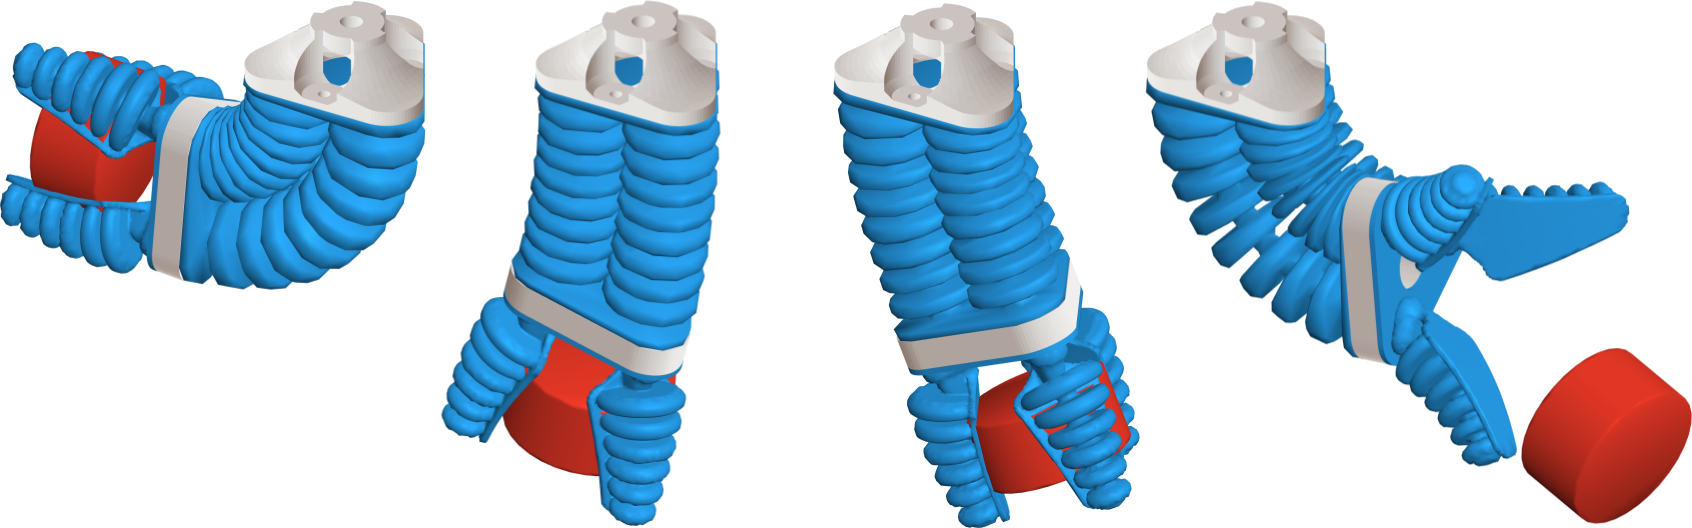
\includegraphics[width=0.95\textwidth]{./pdf/thesis-figure-6-16.png}
\caption{\small Simulation of the soft robot manipulator with gripper using the \class{Shapes} and \class{Model} class. The rigid-body is modeled by the Newton-Euler equation of motions implemented via \class{StateSpace}. }    
\label{fig:C5:srm_simu}
\vspace{-5mm}
\end{figure}
\clearpage
}
    
\subsection{Computer vision (\texttt{Vision})}
\label{sec:C5:vision}
The final Object-oriented class addresses the challenge of soft sensing through vision. The class, named \class{Vision}, can be instantiated using \code{cam = Vision(Id)}, where \code{Id} is a user-specified index obtained from the list of available webcams using \texttt{webcamlist}. Alternatively, the \class{Vision} class is capable of reading sensor data from the RealSense D400 series RGB-Depth camera from Intel. The class is equipped with a suite of vision techniques that make use of the \texttt{OpenCV} Python implementation. It features three key functions: $(i)$ extraction of optical markers from an image using RGB and depth data, $(ii)$ calibration of the world coordinate frame using Aruco markers, and $(iii)$ monitoring of a soft robot in real-time using camera feedback. The detection of color markers utilizes a circular Hough transform \cite{Illingworth1987Sep}, which provides the pixel location of a circle within the specified search conditions. These tools provide a broad range of options for state estimation of a soft robot, which can be easily incorporated into closed-loop control schemes.

